\chapter{Постановка задачи}
\label{section:problem_formulation}

\begin{figure}[htbp]
    \centering
    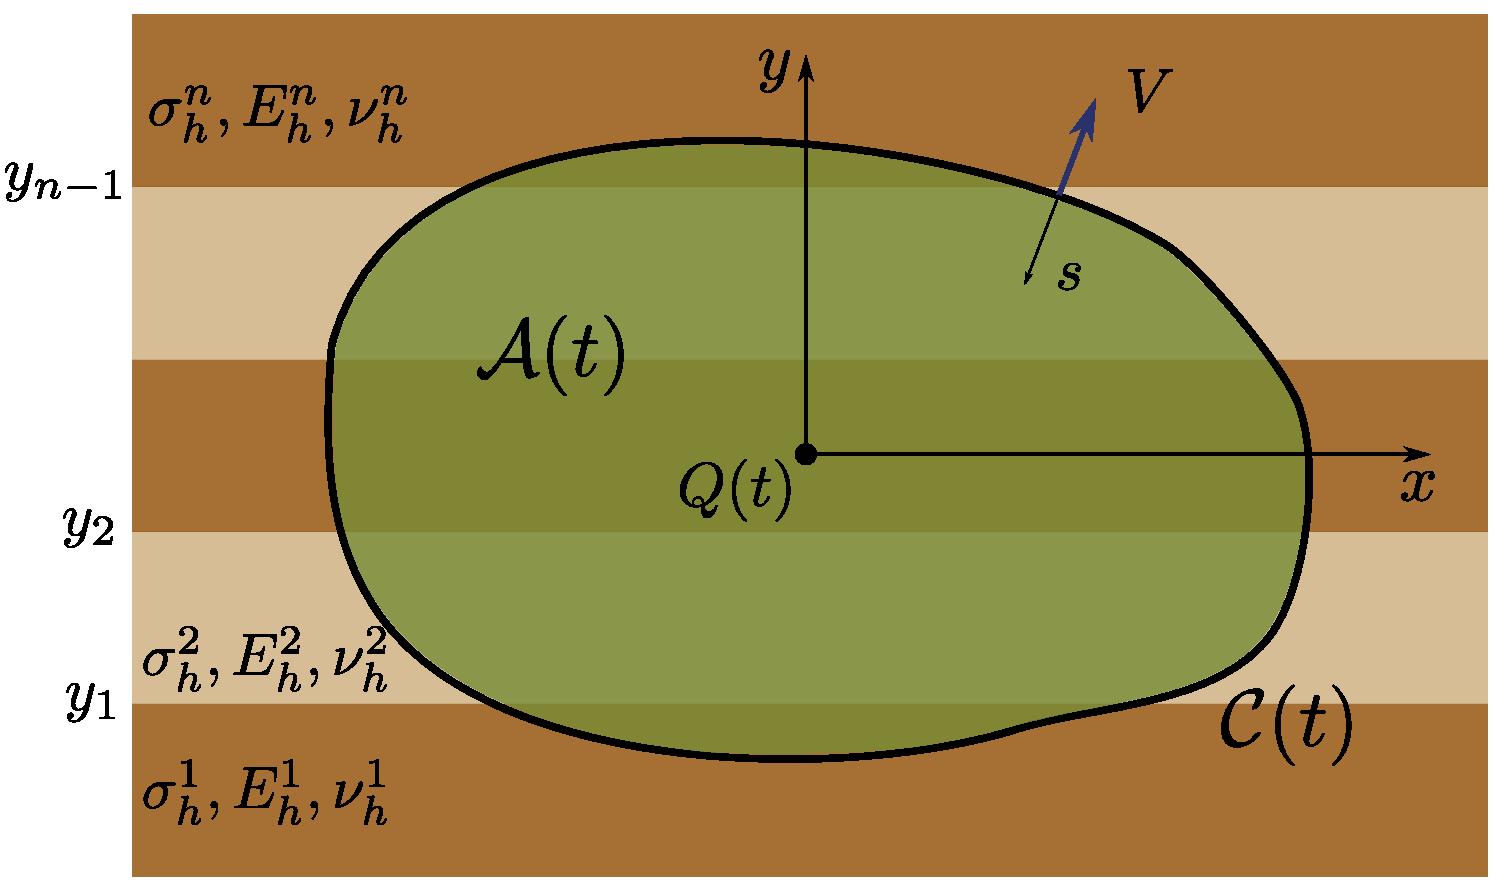
\includegraphics[width=0.7\textwidth]{fracture_scheme.pdf}
    \caption{Модель плоской трещины.}
    \label{fig:planar_fracture}
\end{figure}

Уравнение неразрывности в приближении тонкого слоя для плоской трещины (рисунок~\ref{fig:planar_fracture}) имеет вид
\begin{equation}
    \label{eq:conservation_law}
    \pd{w}{t} + \bigtriangledown \cdot q + \frac{2C_L}{\sqrt{t-t_0(x,\, y)}}  = Q(t) \delta(x,\,y),
\end{equation}
где $w(x,y,t)$ -- раскрытие трещины, $q(x,y,t)$ -- поток жидкости внутри трещины, $Q(t)$ -- объём закаченной в трещину жидкости. Утечки жидкости вычисляются согласно модели Картера~\cite{Cart1957}. $t_0(x,\, y)$ -- момент времени, в который фронт трещины находился в точке $(x, y)$.

Используя закон Пуазейля $q  = -\frac{w^3}{12\mu} \bigtriangledown\! p$ получим уравнение Рейнольдса \cite{DONTSOV201753}
\begin{equation}
    \label{eq:reynolds_equation}
    \pd{w}{t} - \text{div} \left( -\frac{w^3}{12\mu} \bigtriangledown \!p \right) + \frac{2C_L}{\sqrt{t-t_0(x,\, y)}}  = Q(t) \delta(x,\,y),
\end{equation}
где $\mu$ -- вязкость жидкости, $p(x,y,t)$ -- давление жидкости, действующее на поверхности трещины.

Уравнение упругости связывает раскрытие трещины $w$ с давлением $p$
\begin{equation}
    \label{eq:elasticity_equation}
    p(x,y,t) = \sigma_h(y) + \int\limits_{\mathcal{A}(t)} G(x,y;x',y')w(x',y',t) \dif x' \dif y',
\end{equation} 
где $\mathcal{A}(t)$ -- площадь плоской трещины, $\sigma_h$ -- сжимающие напряжение. В случае изотропной среды
\begin{equation}
    \label{eq:elasticity_kernel}
    G(x,y;x',y') = - \frac{E'}{8\pi [(x\!-\!x')^2+(y\!-\!y')^2]^{3/2}}.
\end{equation}
$E' = E / (1-\nu^2)$, где $E$ -- модуль Юнга, $\nu$ -- коэффициент Пуассона.

В случае неоднородности модулей упругости по слоям ядро $G(x,y;x',y')$ не имеет аналитический вид, и для его нахождения требуется численное построение.

Дискретизация уравнений \eqref{eq:reynolds_equation} и \eqref{eq:elasticity_equation} осуществляется с помощью МРС \cite{dispalecement_discontinuty_Crouch1983}. Для этого область разбивается на элементы $\mathcal{A}_{i,j}$ с помощью прямоугольной сетки. Центр ячейки $\mathcal{A}_{i,j}$ расположен в $(x_i,y_j)$ и имеет размеры $\Delta x$, $\Delta y$. Для раскрытия трещины $w$ и давления $p$ используется кусочно-постоянная аппроксимация
\begin{equation}
    \label{eq:piecewiece_approximation}
    \begin{split}
        w(x,y,t) &= \sum\limits_{i,j} w_{i,j}(t) H_{i,j}(x,y), \\
        p(x,y,t) &= \sum\limits_{i,j} p_{i,j}(t) H_{i,j}(x,y), \\
    \end{split}
\end{equation}
где 
\begin{equation}
    \label{eq:heaviside_function}
    H_{i,j}(x,y) = \left\{
        \begin{array}{ll}
            1, & (x,y) \in \mathcal{A}_{i,j}, \\
            0, & (x,y) \notin \mathcal{A}_{i,j}.
        \end{array}\right.
\end{equation}

Тогда уравнение упругости \eqref{eq:elasticity_equation} путём явного интегрирования по элементу сводится к
\begin{equation}
    \label{eq:discrete_elasticity}
    p_{i,j}(t) = {\sigma_h}_{i,j} + \sum\limits_{k,l} C_{i,j;k,l} w_{k,l}(t),
\end{equation}
где $C_{i,j;k,l}$ -- матрица упругости. Дискретизация уравнения Рейнольдса \eqref{eq:reynolds_equation} осуществляется путем интегрирования по времени и элементу \cite{DONTSOV201753}.